
\chapter{Results and Discussion}
In this chapter, the data generated from the experiments presented in the previous chapter are analyzed. The preprocessing methods used on the data is discussed, the metrics used in evaluating the correspondence between image detections and lidar data are introduced, and the results from each experiment are presented. At the end, the detections for each sensor are discussed, and the processing performance of Faster R-CNN is presented.
\section{Post-processing}
In order to associate boat detections in the images to world coordinates, the inverse calibration matrix from equation \ref{eq:calibr} using the values found for the matrix $\mathcal{K}$ in section \ref{section:matlab_calibration} was multiplied with the pixel coordinates of the center point of the bounding boxes found by the faster R-CNN implementation. This associates the pixel coordinates with the normalized image plane presented in figure \ref{fig:image_coordinates} in section \ref{section:camera_coordinates}, giving a direction to the center of the bounding box valid up to a scale factor. Due to the image data being in 2D coordinates, one is only able to associate a detection in an image with a direction, or ray, in 3D space. This ray was subsequently transformed from the camera frame, denoted $c$, to the lidar frame of reference, denoted $l$, using the rotation matrix
\begin{equation}
\mathcal{R}_c^l=\begin{bmatrix}
\cos{\frac{\pi}{2}} & -\sin{\frac{\pi}{2}} & 0 \\
\sin{\frac{\pi}{2}} & \cos{\frac{\pi}{2}} & 0 \\
0 & 0 & 1
\end{bmatrix}\begin{bmatrix}
\cos{-\frac{\pi}{2}} & 0 & \sin{-\frac{\pi}{2}}\\
0 & 1 & 0 \\
-\sin{-\frac{\pi}{2}} & 0 & \cos{-\frac{\pi}{2}}
\end{bmatrix}=\begin{bmatrix}
0 & 0 & 1\\
-1 & 0 & 0\\
0 & -1 & 0
\end{bmatrix}
\end{equation}
which is a rotation of $\frac{\pi}{2}$ radians around the cameras z-axis, followed by a rotation of $-\frac{\pi}{2}$ radians around the new y-axis, and the translation vector
\begin{equation}
\mathbf{t_c^l}=\begin{bmatrix}
0.05 & 0 & -0.097
\end{bmatrix}^T
\end{equation} 
given in meters. The rotation angles and translation vector were measured by hand.

The location used in the experiments gave many returns in the lidar point cloud from the surroundings, which can be considered clutter or noise in the measurements when the task is locating the boat. Figure \ref{fig:ravnkloa_pointcloud} shows a point cloud of the surroundings projected down to two dimensions, illustrating the many unwanted returns. The red circle indicates the area where the maneuvers were performed. The color of the points indicate the height of the point (the z-component for the point), from blue for the lowest points, to yellow for the highest.
\begin{figure}[!htb]
	\centering
	\includegraphics[width=\linewidth]{fig/ravnkloa_surroundings.png}
	\caption{The lidar point cloud including surroundings at Ravnkloa, projected down to the xy-plane.}
	\label{fig:ravnkloa_pointcloud}
\end{figure}
The returns from the boat in the lidar data was compared with detections from the Faster R-CNN network. In order to remove all returns from the lidar that were known to originate from the surroundings were removed, using a "pass through" filter removing all points which lies outside a specified rectangular region in the xy-plane, keeping only the returns from the designated testing area. The point cloud was also reduced to two dimensions by projecting all points down to the plane $z=0$. In addition, the point cloud returns were limited in post-processing to only those lying in the cameras field of view.
Once the point cloud was reduced to two dimensions, and all returns originating from the surroundings were removed, k-Means clustering (with k=1) was used to find the centroid of the points returned by the boat.
An overview of the post-processing pipeline is given in figure \ref{fig:post_pipeline}.
\begin{figure}[!htb]
	\centering
	\includegraphics[width=.8\linewidth]{fig/post-processing-pipeline.pdf}
	\caption{The data post-processing pipeline.}
	\label{fig:post_pipeline}
\end{figure}
An example of a image detection associated with the point cloud cluster center is shown in figure \ref{fig:sub_proj_ex1}. The line from the origin to the cluster center is the projection of the bounding box centroid of the detected boat in the image. The corresponding image generating the detection is shown in figure \ref{fig:sub_proj_ex2}.
\begin{figure}[H]
		\centering
		\includegraphics[width=\linewidth]{fig/proj_example.png}
		\caption{Point cloud cluster, with image detection drawn in.}
		\label{fig:sub_proj_ex1}
\end{figure}%
\begin{figure}[H]
		\centering
		\includegraphics[width=\linewidth]{fig/proj_example_im.png}
		\caption{Image from the camera, with bounding boxes corresponding to detected boats overlaid.}
		\label{fig:sub_proj_ex2}
\end{figure}

\section{Metrics}
Faster R-CNN gives the bounding boxes for its detections, along with the score for the detection, indicating the "confidence" in the classification. The threshold for the score was set to 0.6, where 1.0 indicates absolute certainty (from the detectors perspective) and 0 indicates zero confidence. The 0.6 threshold was the default set in the faster R-CNN implementation from the Github repository. The detection threshold has not been analyzed with particular attention in this project.

As a metric in determining whether or not a detection from the convolutional net corresponds with the boat, the minimum distance between the ray projected by the centroid of the bounding box and the centroid of the point cloud cluster corresponding to the boat was used. This distance was set to 2.5 meters, which is approximately half the length of the boat used in the experiments. This value was heuristically determined through experimentation, and was chosen as a compromise between the target boat being detected versus boats in the background counting as a detection of the target boat. Due to the geometry of the boat, for some maneuvers the majority of the returns found by the lidar come from the front part of the boat, while the detections in the image are more centered on the projection of the boat into the image plane. The 2.5 meters distance also allow for some time difference between the images and the point cloud, as the data is not time stamped at capture time, but at arrival time in the computer, not accounting for intermediary processing and transmission delay. The images corresponding to a particular point cloud were found by searching through the image set and selecting the image with the temporally closest time stamp, since the time offset between the lidar and the camera is unknown. Lastly, the transformation between the camera frame and the lidar frame is hand-measured and assumes that the camera z-axis is perfectly aligned with the lidar x-axis, not taking into account misalignments. The minimum distance of 2.5 meters allows for some leeway in the alignment of the sensors. 

In order to avoid multiple detections in cases where the target boat pass in front of a boat in the background, only the detection closest to the point cloud cluster center is considered. For each experiment, the total number of image detections corresponding to a point cloud are calculated. The images counting towards a detection match are examined manually, and if the detection is a false detection caused by the background, or a background ship is detected instead of the target, they are counted as a false detection. The accumulated point cloud cluster centers are plotted as a track for each experiment, and color coded to indicate if there is a detection in a image corresponding to that particular point cloud cluster center.
\section{Experimental Results}
%%%%%%%%%%%%%%%%%%%%%%%%%%%%%%%%%%%%%%%%%%%%%%%%%%%%%%%%%%%%%%%%%%%%%%%%%%%%%%%%%%%%%%%%%%%%%%%%%%%%%%%%%%%%%%%%%%%%%
\subsection{Experiment 1}
Experiment 1 was performed by the vessel arriving head on towards the sensor setup, see figure \ref{fig:experiments}.
The first return from the boat was attained at a range of 67.39 meters, which is the rightmost cluster in figure \ref{fig:ex1_track}. The image corresponding to this cluster is shown in \ref{fig:ex1_1}.
\begin{figure}[h]
		\centering
		\includegraphics[width=\linewidth]{fig/detection_1_exp_1_img.png}
		\caption{Image corresponding to the first lidar return, with bounding boxes overlaid. The target is the smallest rectangle in the center of the image.}
		\label{fig:ex1_1}
\end{figure}

\begin{figure}[H]
	\centering
	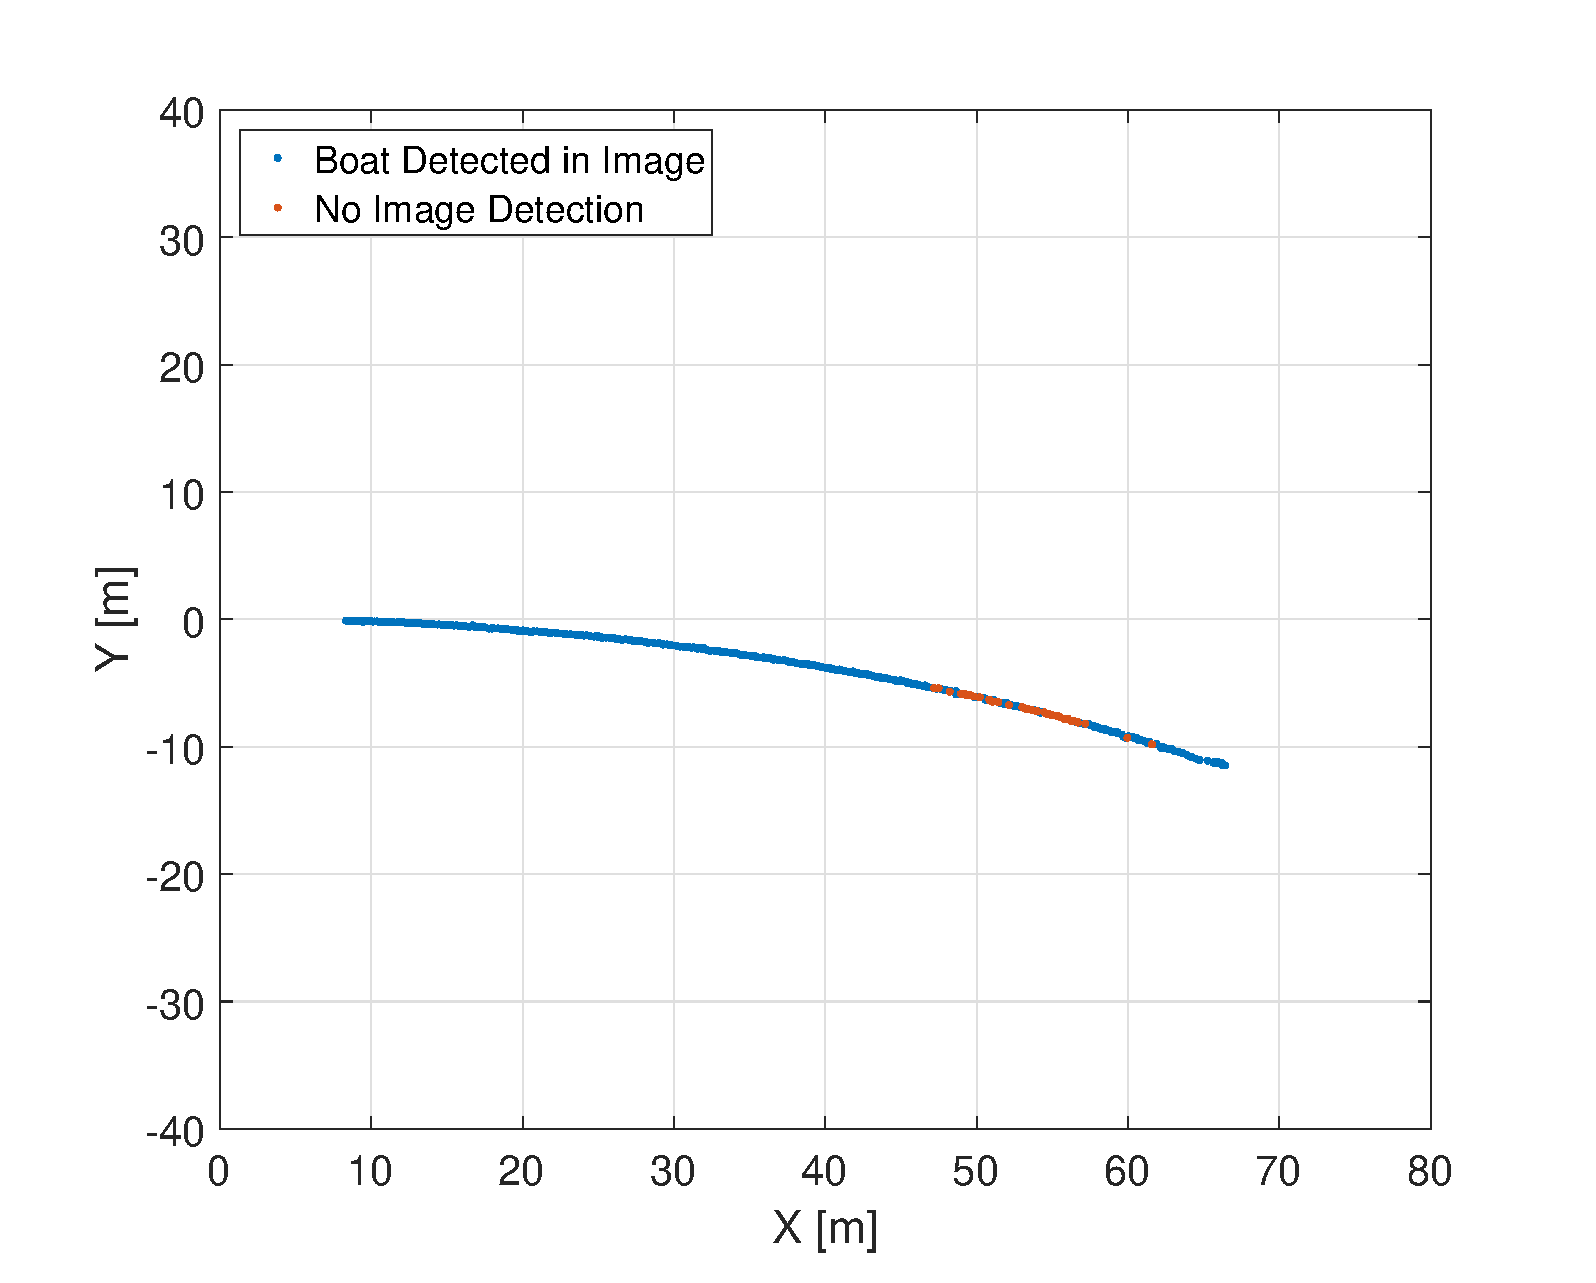
\includegraphics[width=.8\linewidth]{fig/exp_1_track.eps}
	\caption{Track generated by point cloud cluster center in experiment 1.}
	\label{fig:ex1_track}
\end{figure}
As seen in figure \ref{fig:ex1_track}, there are some missed detections in the image data around $x=50$ meters.
Looking at figure \ref{fig:ex1_50m}, where the boat is at approximately $x=50$ meters, it's hard to determine an exact reason for this. One possibility may be that a combination of lighting conditions and background kept the detection score below the threshold of 0.6 for some time.
\begin{figure}[H]
	\centering
	\includegraphics[width=\linewidth]{fig/exp1_bb_50m.png}
	\caption{Missed detection in experiment 1.}
	\label{fig:ex1_50m}
\end{figure}
As figure \ref{fig:ex1_track} shows, once the vessel was within 40 meters, every single point cloud had a corresponding detection of the vessel. The total number of point clouds, total number of detections, the fraction of boat detections in images over the total number of point clouds, and the number of false image detections for experiment 1 is shown in table \ref{tab:exp1}. There were no image detections not originating from the target boat in experiment 1.
\begin{table}[H]
	\centering
	\begin{tabularx}{.7\linewidth}{L c}
		\toprule
		Number of point clouds & 409\\
		\midrule
		Number of detections & 365\\
		\midrule
	    Detections/Point clouds & 0.8924 \\
	    \midrule
	    False detections & 0\\
		\bottomrule
	\end{tabularx}
\caption{Data from experiment 1.}
\label{tab:exp1}
\end{table}
%%%%%%%%%%%%%%%%%%%%%%%%%%%%%%%%%%%%%%%%%%%%%%%%%%%%%%%%%%%%%%%%%%%%%%%%%%%%%%%%%%%%%%%%%%%%%%%%%%%%%%%%%%%%%%%%%%%%%
\subsection{Experiment 2}
Experiment 2 was performed by the vessel approaching the sensor location from an angle, see figure \ref{fig:experiments}. The track generated by the point cloud cluster centers are shown in figure \ref{fig:ex2_track}.
\begin{figure}[H]
	\centering
	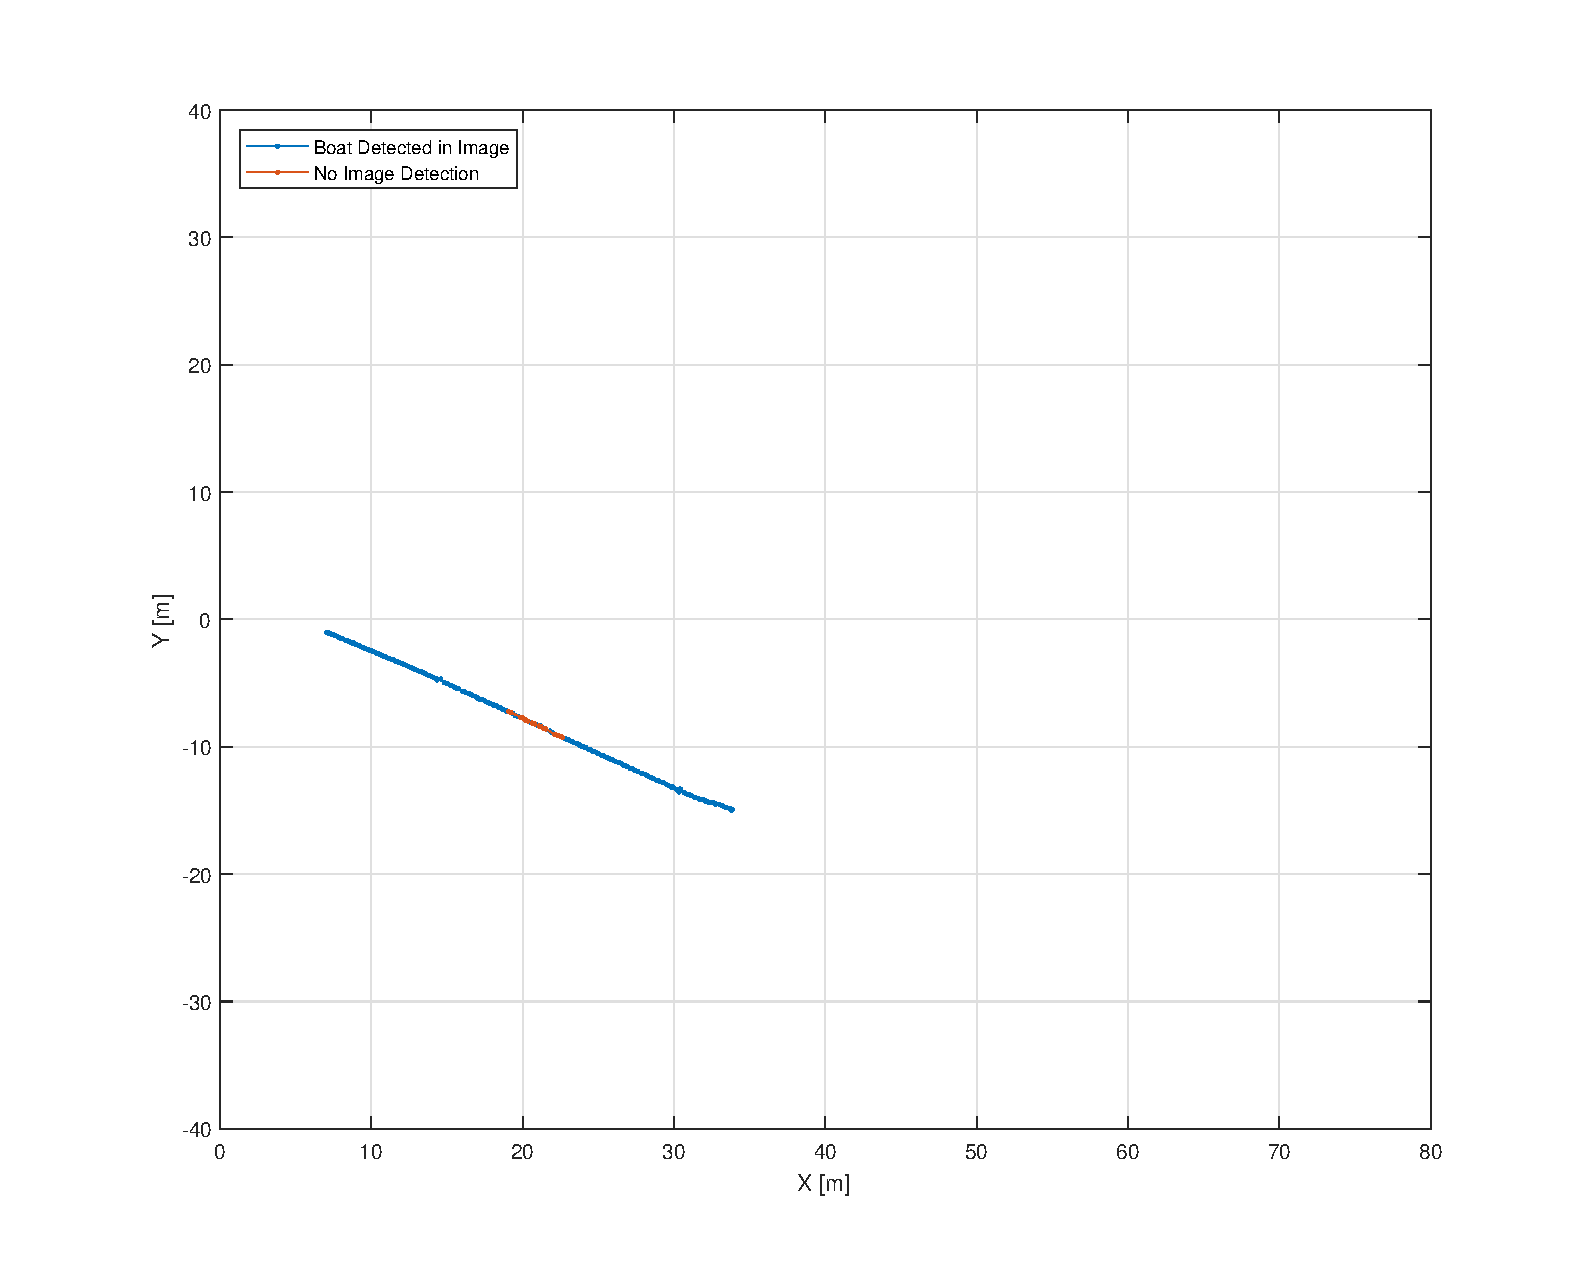
\includegraphics[width=.8\linewidth]{fig/exp_2_track.eps}
	\caption{Track generated by point cloud cluster center in experiment 2.}
	\label{fig:ex2_track}
\end{figure}
As seen in figure \ref{fig:ex2_track}, there is an interval around $x=20$ meters where the image detections dissapear. Figure \ref{fig:sub_ex2_issue} shows the reason for this, as a ship in the background is influencing the detection of the target. In figure \ref{fig:sub_ex2_issue2}, the target vessel has moved enough for the two boats to be detected separately.
\begin{figure}[H]
	\centering
	\begin{subfigure}[t]{.5\linewidth}
		\centering
		\includegraphics[width=\linewidth]{fig/exp_2_problem.png}
		\caption{Background boat interfering with\\ the detection of the target.}
		\label{fig:sub_ex2_issue}
	\end{subfigure}%
	\begin{subfigure}[t]{.5\linewidth}
		\centering
		\includegraphics[width=\linewidth]{fig/exp2_past_problem.png}
		\caption{Large enough separation to be detected as two separate boats.}
		\label{fig:sub_ex2_issue2}
	\end{subfigure}
	\caption{Background ship interfering with the detection of the target.}
	\label{fig:issues_ex2}
\end{figure}
The total number of point clouds, total number of detections, the fraction of boat detections in images over the total number of point clouds, and the number of false image detections for experiment 2 is shown in table \ref{tab:exp2}. The false image detections for experiment 2 occured when the background ship was influencing the detection of the target, as shown in figure \ref{fig:issues_ex2}.
\begin{table}[H]
	\centering
	\begin{tabularx}{.7\linewidth}{L c}
		\toprule
		Number of point clouds & 203\\
		\midrule
		Number of detections & 186\\
		\midrule
		Detections/Point clouds & 0.9163 \\
		\midrule
		False detections & 25\\
		\bottomrule
	\end{tabularx}
	\caption{Data from experiment 2.}
	\label{tab:exp2}
\end{table}

%%%%%%%%%%%%%%%%%%%%%%%%%%%%%%%%%%%%%%%%%%%%%%%%%%%%%%%%%%%%%%%%%%%%%%%%%%%%%%%%%%%%%%%%%%%%%%%%%%%%%%%%%%%%%%%%%%%%%
\subsection{Experiment 3}
Experiment 3 was performed by the boat passing across of the sensors, at a distance of approximately 25 to 15 meters in the $x$-direction. As seen in figure \ref{fig:ex3_track}, the target is detected in almost all of the images corresponding to the point clouds in the track. There are some missed detections near the end of the track, around $x=20$ and $y=10$ in figure \ref{fig:ex3_track}. As seen in figure \ref{fig:issues_ex3}, there are boats in the background at this part of the track. Figure \ref{fig:hit_ex3} shows a good detection of the target.
\begin{figure}[h]
	\centering
	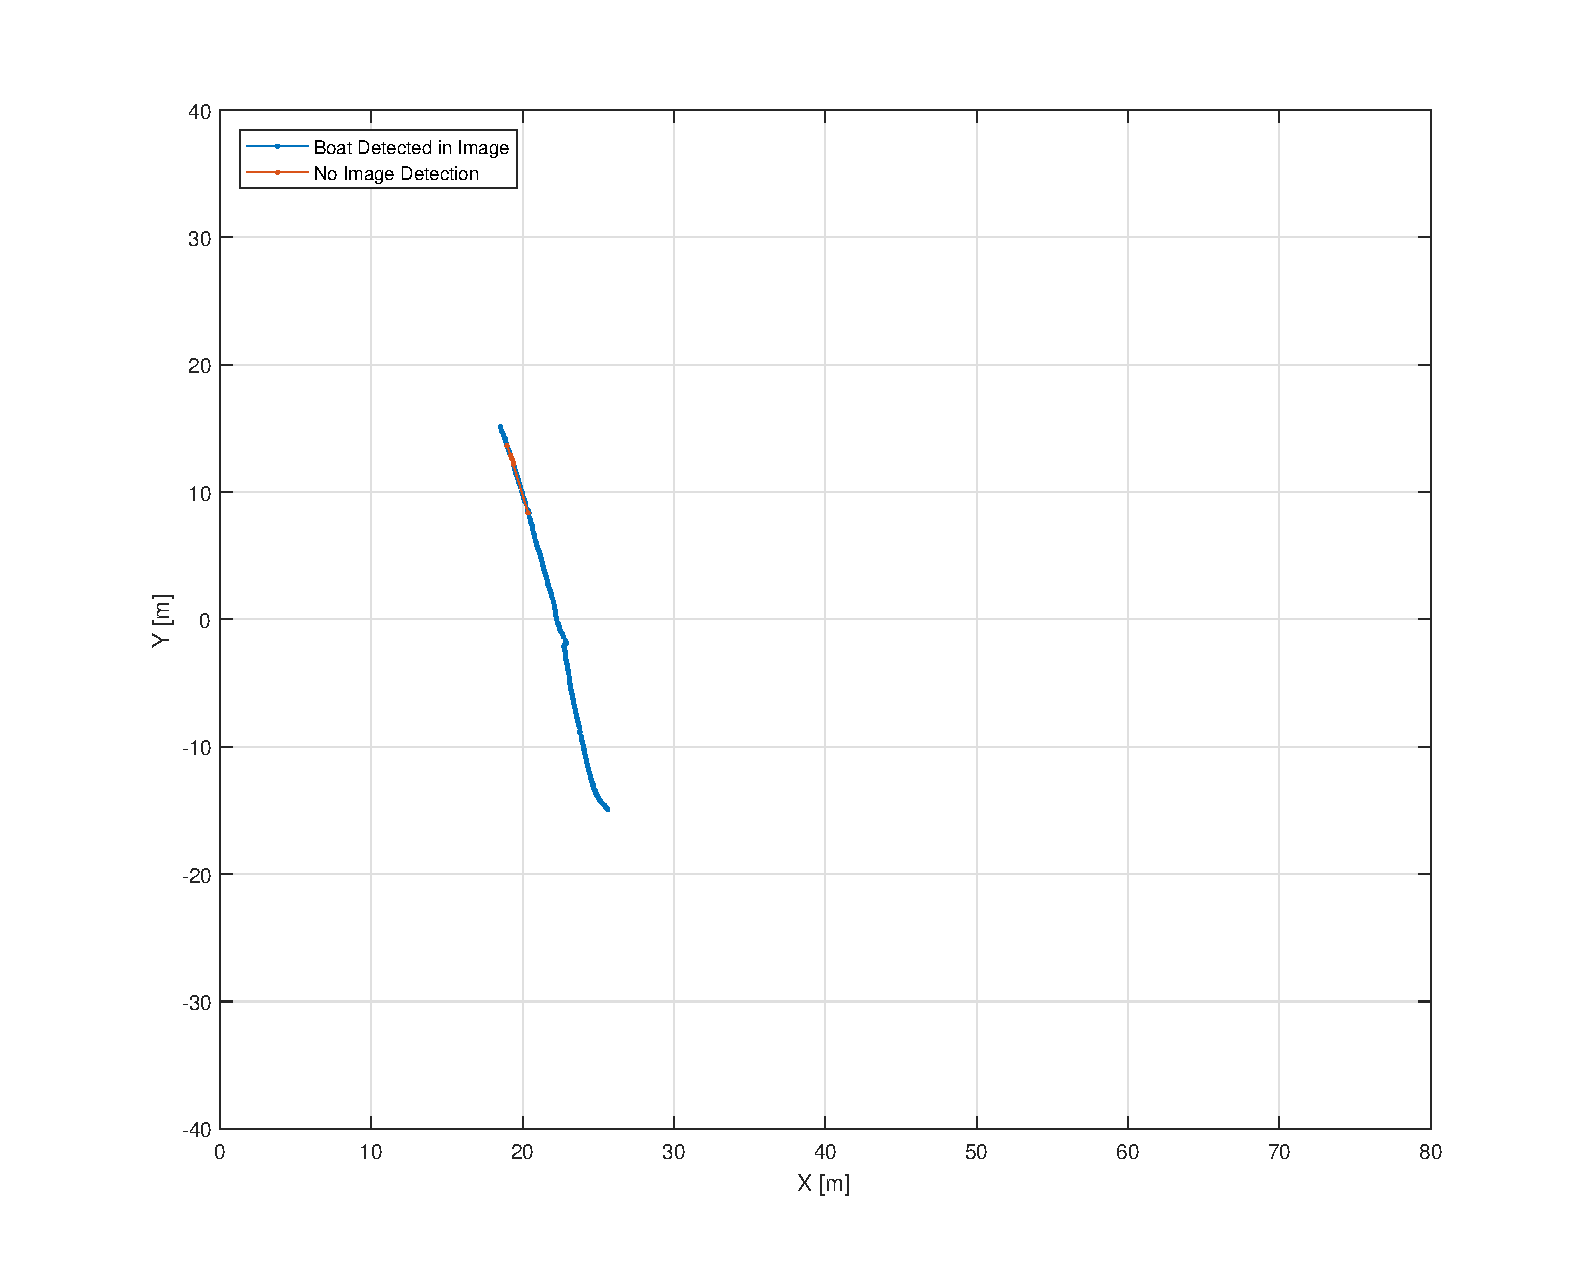
\includegraphics[width=.8\linewidth]{fig/exp_3_track.eps}
	\caption{Track generated by point cloud cluster center in experiment 3.}
	\label{fig:ex3_track}
\end{figure}
\begin{figure}[H]
	\centering
	\includegraphics[width=\linewidth]{fig/ex3_miss.png}
	\caption{Target not detected in the image in experiment 3.}
	\label{fig:issues_ex3}
\end{figure}%
\begin{figure}[H]
	\centering
	\includegraphics[width=\linewidth]{fig/ex3_hit.png}
	\caption{Good detection of the target in experiment 3.}
	\label{fig:hit_ex3}
\end{figure}%
The total number of point clouds, total number of detections, the fraction of boat detections in images over the total number of point clouds, and the number of false image detections for experiment 3 is shown in table \ref{tab:exp3}. All image detections in experiment 3 were found to originate from the target boat.
\begin{table}[h]
	\centering
	\begin{tabularx}{.7\linewidth}{L c}
		\toprule
		Number of point clouds & 214\\
		\midrule
		Number of detections & 207\\
		\midrule
		Detections/Point clouds & 0.9673 \\
		\midrule
		False detections & 0\\
		\bottomrule
	\end{tabularx}
	\caption{Data from experiment 3.}
	\label{tab:exp3}
\end{table}
%%%%%%%%%%%%%%%%%%%%%%%%%%%%%%%%%%%%%%%%%%%%%%%%%%%%%%%%%%%%%%%%%%%%%%%%%%%%%%%%%%%%%%%%%%%%%%%%%%%%%%%%%%%%%%%%%%%%%
\subsection{Experiment 4}
Experiment 4 was performed by the boat passing across the sensor setup, this time at a distance of approximately 30 to 40 meters in the $x$-direction. Figure \ref{fig:ex4_track} shows the track generated by the point cloud cluster centers.
\begin{figure}[!htb]
	\centering
	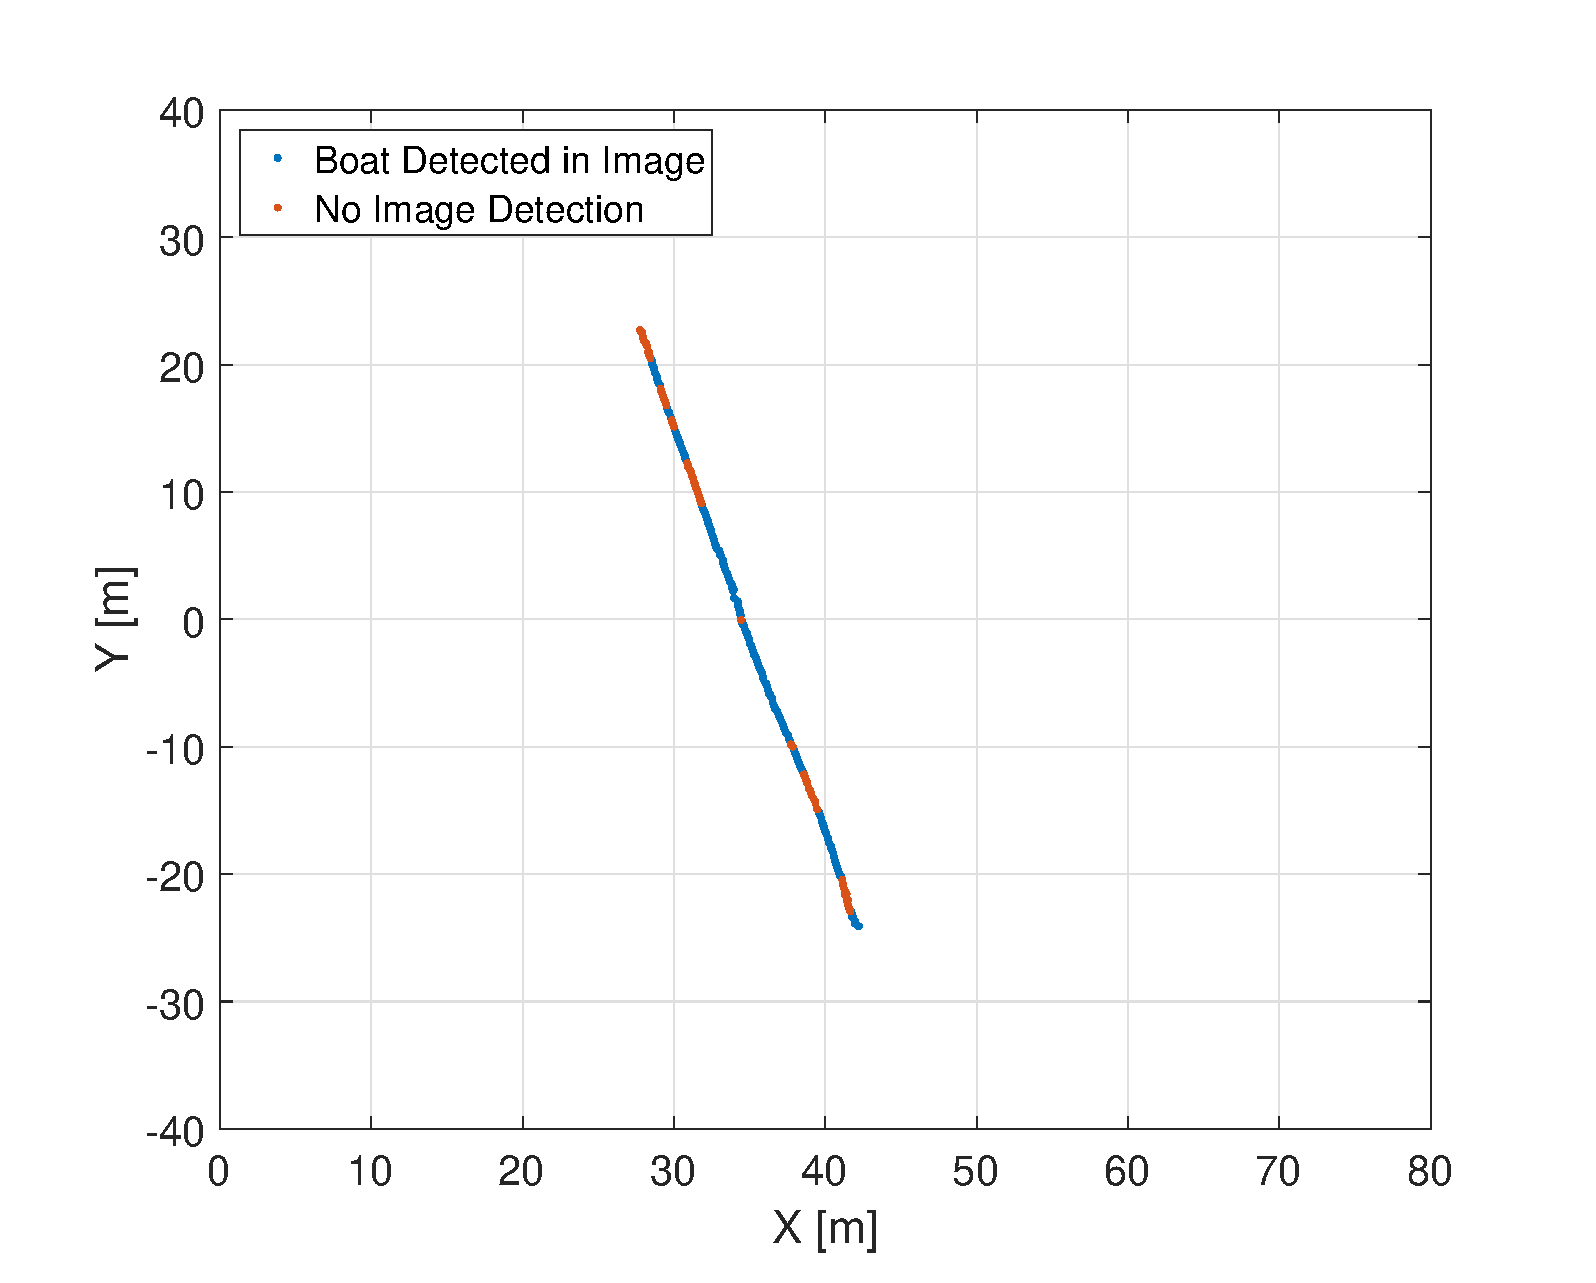
\includegraphics[width=.8\linewidth]{fig/exp_4_track.eps}
	\caption{Track generated by point cloud cluster center in experiment 4.}
	\label{fig:ex4_track}
\end{figure}
Again, we see from figure \ref{fig:ex4_track} that there are certain parts of the track where the image detections suffer. The image in figure \ref{fig:issues_ex4} corresponds to a missed detection at the top of the track in figure \ref{fig:ex4_track}. There are boats in the background of the image at this part of the track, possibly interfering with the detection of the target. Comparing the location of boats in the background in figure \ref{fig:issues_ex4} with the locations where there were no image detections in figure \ref{fig:ex4_track}, we see that for all parts of the track where image detections are missing, there are boats in the background of the image, suggesting that boats in the background might be interfering with the detection of the target throughout the experiment. Closer examination of the dataset shows that this is generally the case, and as seen in figure \ref{fig:issues_ex4_train}, a passing train in the background also confused the detector at one point.
\begin{figure}[!htb]
	\centering
	\includegraphics[width=\linewidth]{fig/ex4_miss.png}
	\caption{Background interfering with the detection of the target in the image in experiment 4.}
	\label{fig:issues_ex4}
\end{figure}
\begin{figure}[!htb]
	\centering
	\includegraphics[width=\linewidth]{fig/ex4_train.png}
	\caption{Train in the background confusing the detection of the target in the image in experiment 4.}
	\label{fig:issues_ex4_train}
\end{figure}

The total number of point clouds, total number of detections, the fraction of boat detections in images over the total number of point clouds, and the number of false image detections for experiment 4 is shown in table \ref{tab:exp4}. The false image detections occured when the target boat was passing in front of the moored boats in the background, as well as one occation where a train in the background influenced the detection, as shown in figure \ref{fig:issues_ex4_train}.
\begin{table}[H]
	\centering
	\begin{tabularx}{.7\linewidth}{L c}
		\toprule
		Number of point clouds & 240\\
		\midrule
		Number of detections & 171\\
		\midrule
		Detections/Point clouds & 0.7125 \\
		\midrule
		False detections & 8\\
		\bottomrule
	\end{tabularx}
	\caption{Data from experiment 4.}
	\label{tab:exp4}
\end{table}
%%%%%%%%%%%%%%%%%%%%%%%%%%%%%%%%%%%%%%%%%%%%%%%%%%%%%%%%%%%%%%%%%%%%%%%%%%%%%%%%%%%%%%%%%%%%%%%%%%%%%%%%%%%%%%%%%%%%%
\subsection{Experiment 5}
In experiment 5, the boat was passing across the sensor setup at a distance of approximately 45 to 30 meters in the $x$-direction, this time with a speed of approximately 2.5 meters/second. As seen in figure \ref{fig:ex5_track}, this experiment generated few image detections, compared to the previous experiments. This is again partly due to background interference as can be seen in figures \ref{fig:ex5_multiple_1} and \ref{fig:ex5_multiple_2}, as well as parts where the boat was simply not detected, as shown in figure \ref{fig:ex5_miss}.
\begin{figure}[!htb]
	\centering
	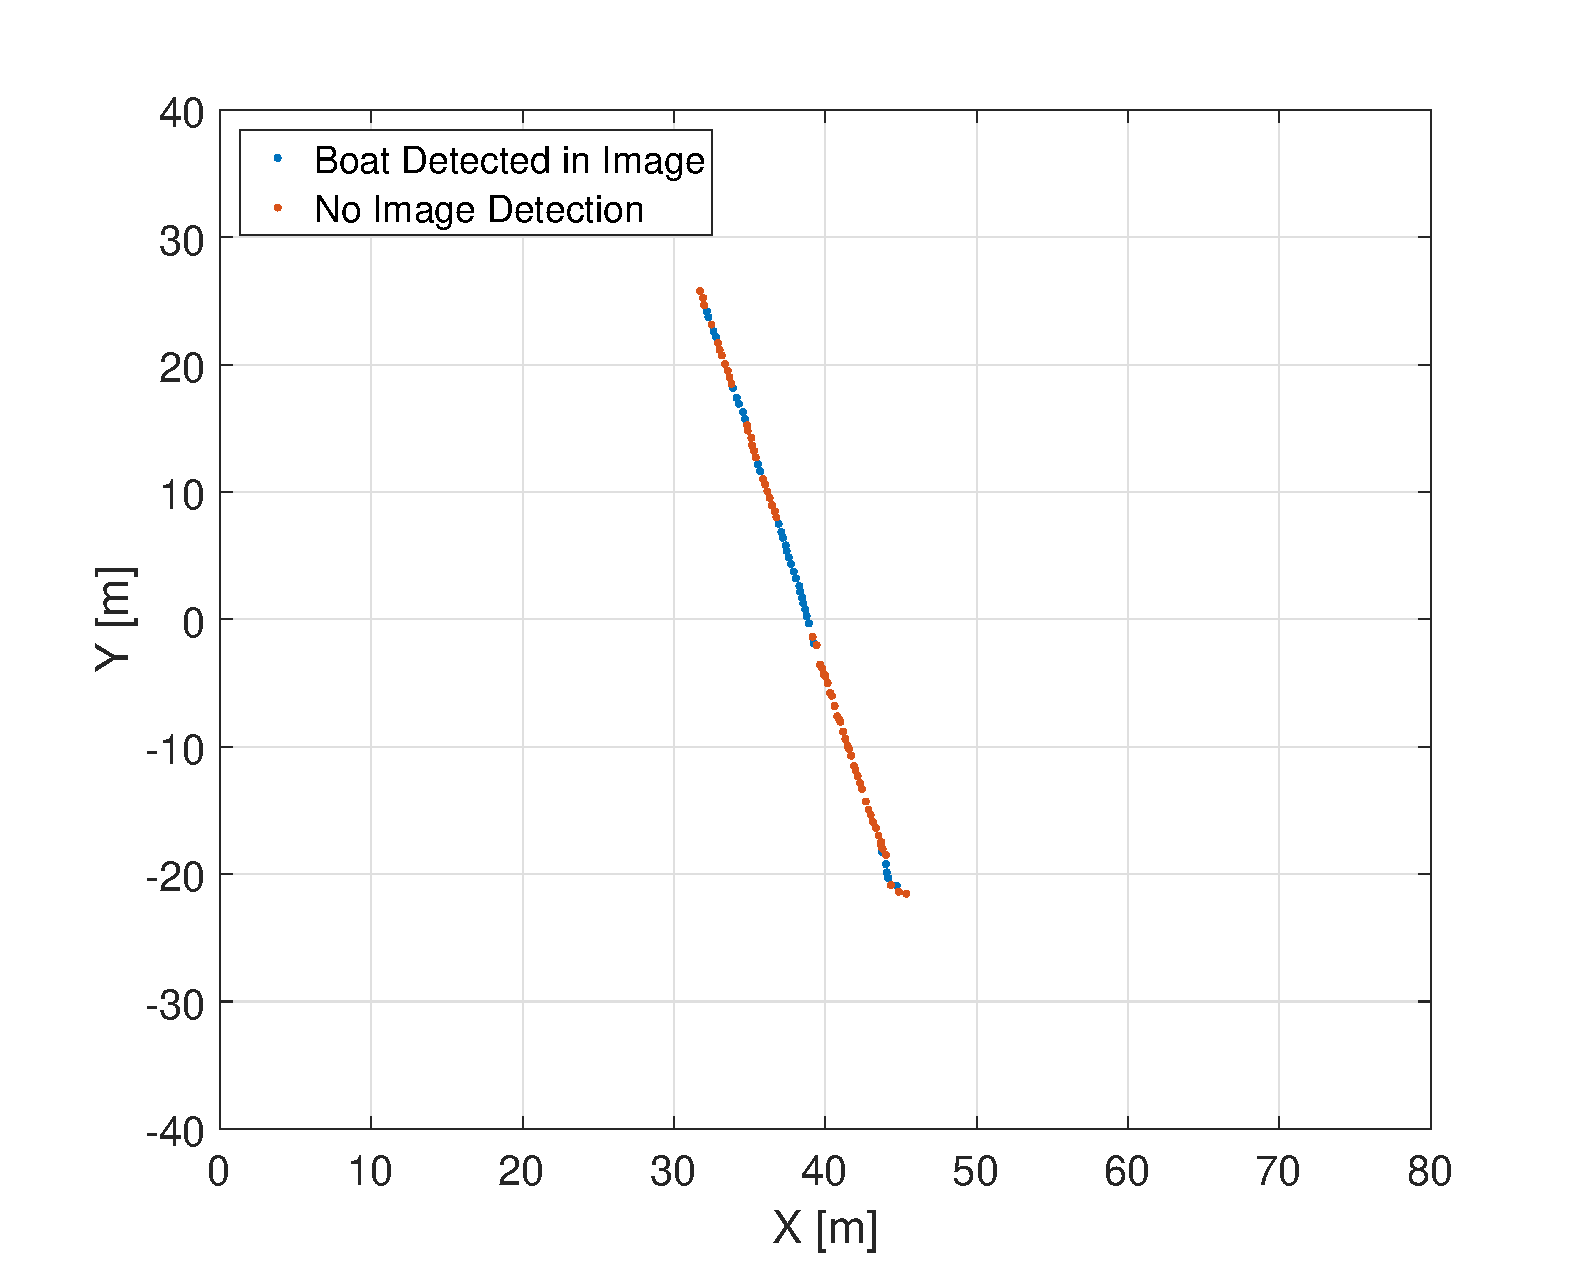
\includegraphics[width=.8\linewidth]{fig/exp_5_track.eps}
	\caption{Track generated by point cloud cluster center in experiment 5.}
	\label{fig:ex5_track}
\end{figure}
\begin{figure}[h]
	\centering
	\includegraphics[width=\linewidth]{fig/ex5_multiple_2.png}
	\caption{Background interfering with detection in experiment 5, example 1. Target can be seen in the center of the image, just to the right of the bridge crossing in the background.}
	\label{fig:ex5_multiple_1}
\end{figure}%
\begin{figure}[h]
	\centering
	\includegraphics[width=\linewidth]{fig/ex5_multiple.png}
	\caption{Background interfering with detection in experiment 5, example 2. Target can be seen just below the tall tower in the background, in the leftmost part of the image.}
	\label{fig:ex5_multiple_2}
\end{figure}%
\begin{figure}[H]
		\centering
		\includegraphics[width=\linewidth]{fig/ex5_no_hit.png}
		\caption{Target boat not detected. Target can be seen in the center of the image.}
		\label{fig:ex5_miss}
\end{figure}%

The total number of point clouds, total number of detections, the fraction of boat detections in images over the total number of point clouds, and the number of false image detections for experiment 5 is shown in table \ref{tab:exp5}. The false image detections occured again when the target was passing the boats in the background.
\begin{table}[H]
	\centering
	\begin{tabularx}{.7\linewidth}{L c}
		\toprule
		Number of point clouds & 94\\
		\midrule
		Number of detections & 33\\
		\midrule
		Detections/Point clouds & 0.3511 \\
		\midrule
		False detections & 7\\
		\bottomrule
	\end{tabularx}
	\caption{Data from experiment 5.}
	\label{tab:exp5}
\end{table}
%%%%%%%%%%%%%%%%%%%%%%%%%%%%%%%%%%%%%%%%%%%%%%%%%%%%%%%%%%%%%%%%%%%%%%%%%%%%%%%%%%%%%%%%%%%%%%%%%%%%%%%%%%%%%%%%%%%%%
\subsection{Experiment 6}
In experiment 6, the boat was passing across the sensor setup at a distance between approximately 45 to 65 meters in the $x$-direction. Figure \ref{fig:ex6_track} shows the recorded track for this experiment.  
\begin{figure}[!htb]
	\centering
	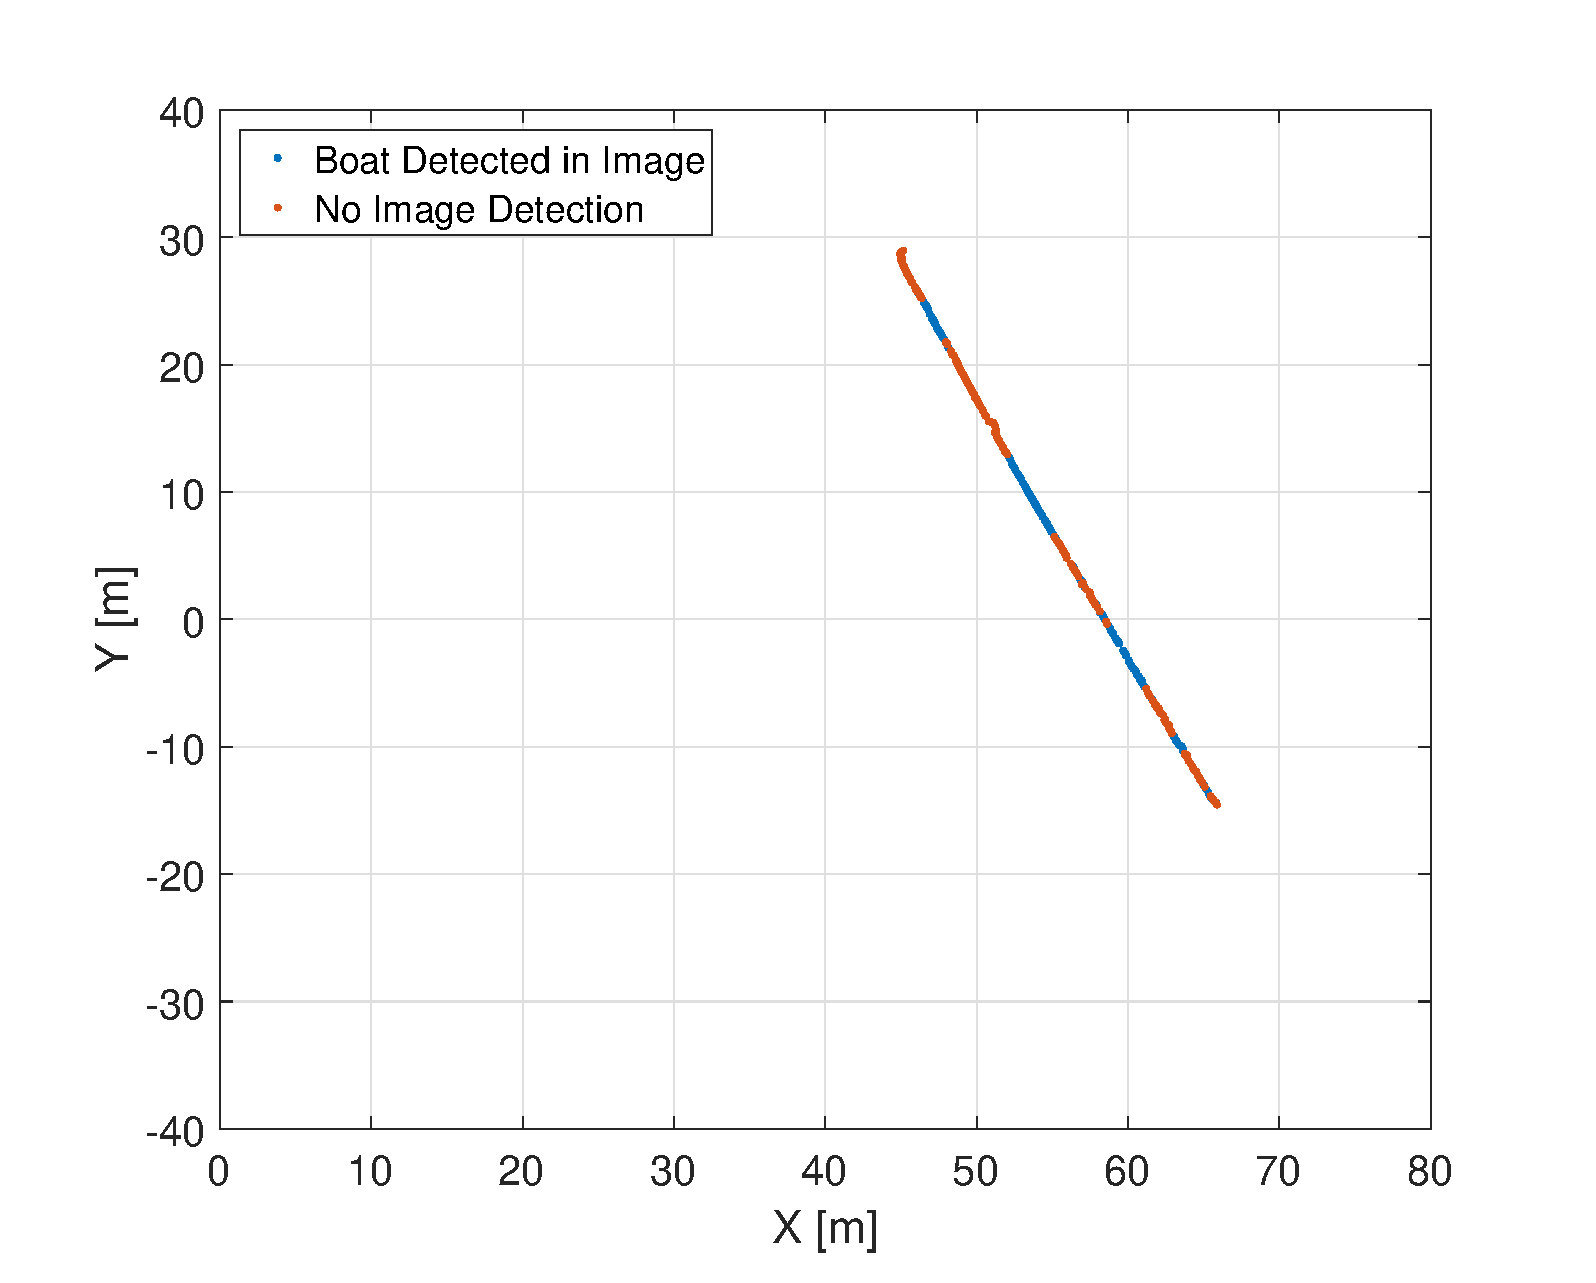
\includegraphics[width=.8\linewidth]{fig/exp_6_track.eps}
	\caption{Track generated by point cloud cluster center in experiment 6.}
	\label{fig:ex6_track}
\end{figure}

This experiment also has a lot of missed detections in the image data. Figure \ref{fig:issues_ex6} shows a case where the target is passing a moored boat in the background, where actual detection is that of the background boat, falsely counting towards a detection of the target due to the bounding box center falling within the minimum distance from the point cloud cluster center. Figure \ref{fig:issues_ex6_2} shows a case where the target boat is not detected in the image, while figure \ref{fig:issues_ex6_3} shows a case where the target is correctly detected.
\begin{figure}[!htb]
	\centering
	\includegraphics[width=\linewidth]{fig/ex6_hit.png}
	\caption{Target correctly detected in image in experiment 6. Target is within bounding box number four, counting from the left.}
	\label{fig:issues_ex6_3}
\end{figure}
\begin{figure}[H]
	\centering
	\includegraphics[width=\linewidth]{fig/ex6_false.png}
	\caption{Leftmost background boat detection falsely counted as target detection in experiment 6.}
	\label{fig:issues_ex6}
\end{figure}
\begin{figure}[H]
	\centering
	\includegraphics[width=\linewidth]{fig/ex6_miss.png}
	\caption{Target not detected in image in experiment 6. Target can be seen between bounding boxes two and three, counting from the left.}
	\label{fig:issues_ex6_2}
\end{figure}
The total number of point clouds, total number of detections, the fraction of boat detections in images over the total number of point clouds, and the number of false image detections for experiment 6 is shown in table \ref{tab:exp6}. The false detections in the images occured at the start of the track, when the target boat was passing in front of the boats in the background.
\begin{table}[!htb]
	\centering
	\begin{tabularx}{.7\linewidth}{L c}
		\toprule
		Number of point clouds & 266\\
		\midrule
		Number of detections & 114\\
		\midrule
		Detections/Point clouds & 0.4286 \\
		\midrule
		False detections & 25\\
		\bottomrule
	\end{tabularx}
	\caption{Data from experiment 6.}
	\label{tab:exp6}
\end{table}
%%%%%%%%%%%%%%%%%%%%%%%%%%%%%%%%%%%%%%%%%%%%%%%%%%%%%%%%%%%%%%%%%%%%%%%%%%%%%%%%%%%%%%%%%%%%%%%%%%%%%%%%%%%%%%%%%%%%%
\subsection{Experiment 7}
In experiment 7, the boat moved in a circular pattern, as seen in the track in figure \ref{fig:ex7_track}. The start of the track, and the experiment, is the top most data point in figure \ref{fig:ex7_track}, subsequently entering the circular pattern. The boat completed three full circles during the experiment. As seen in the track in figure \ref{fig:ex7_track}, the missed image detections occur at the same part of the track for each completed circle, at both sides of the circle lying on a ray originating in the origin, as well as at the top of the circle in figure \ref{fig:ex7_track}. The missed image detections at the start of the track is due to the boat not being fully in the field of view of the camera at the start of the recording.
\begin{figure}[!htb]
	\centering
	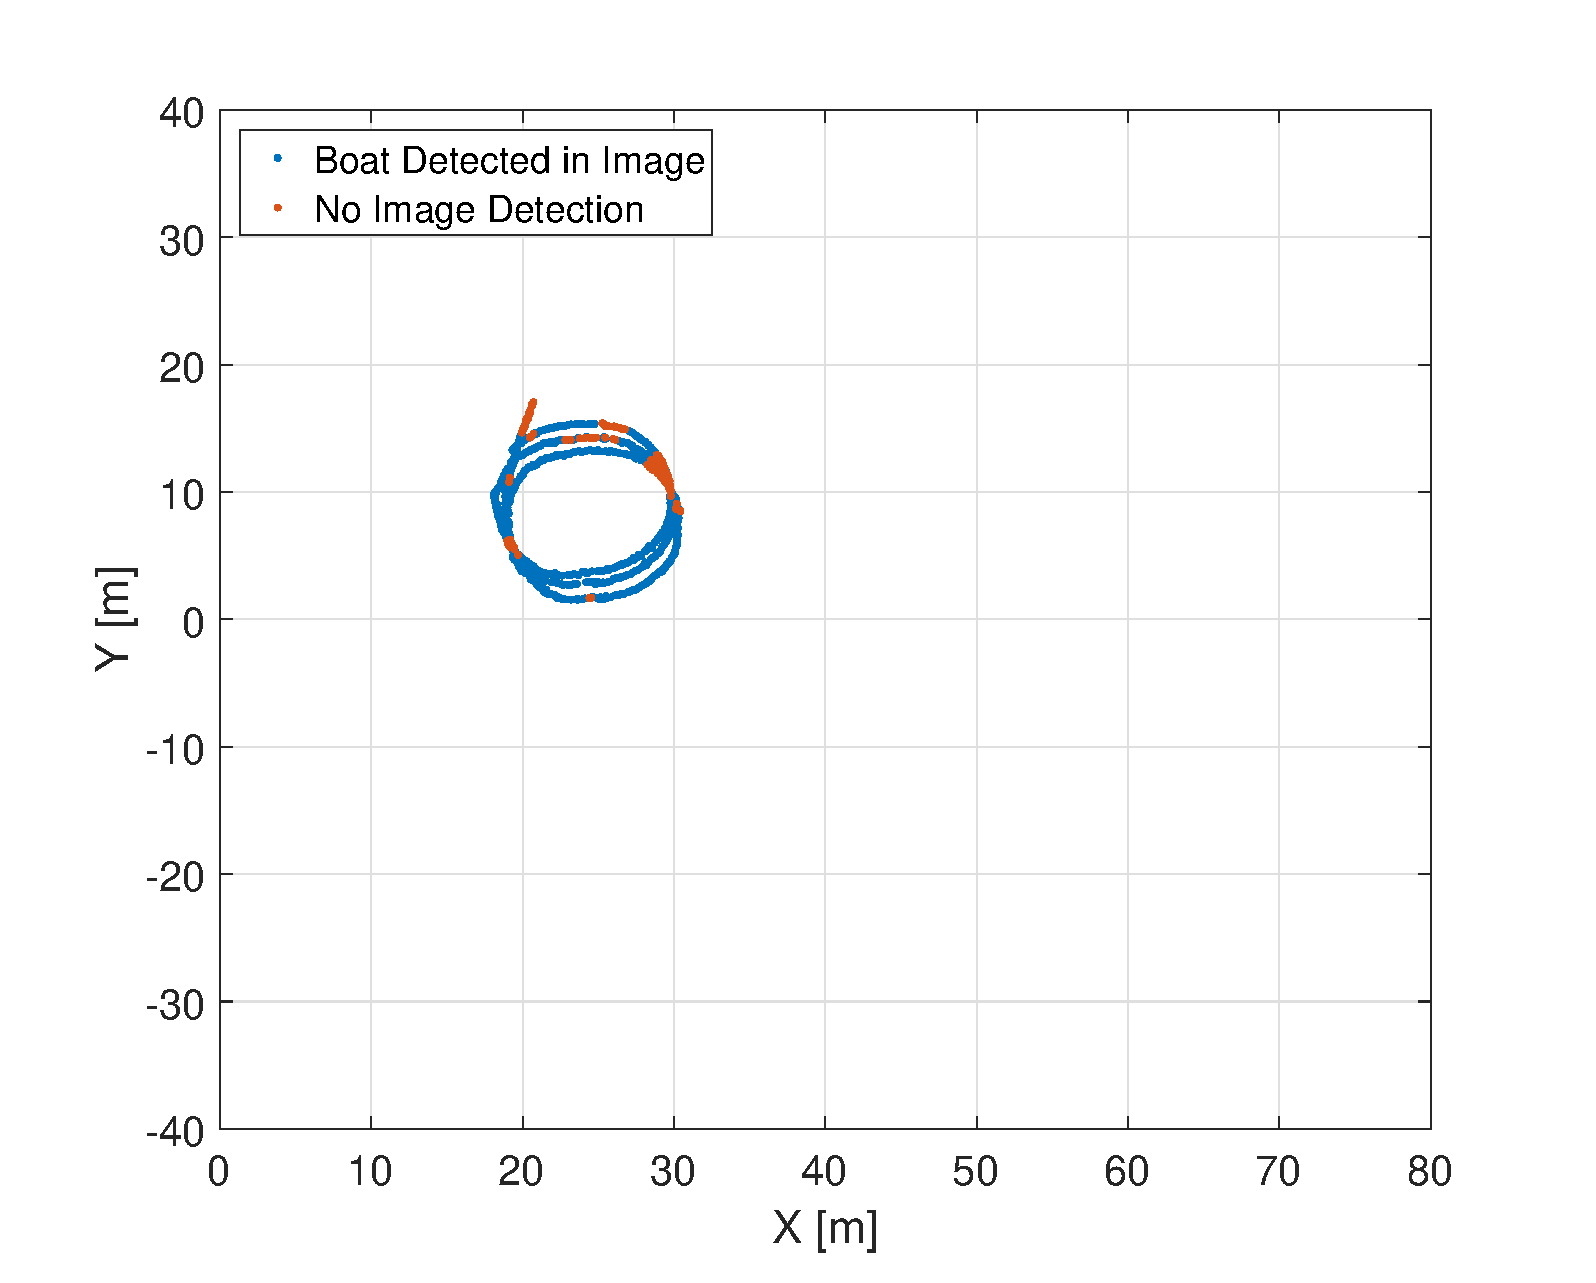
\includegraphics[width=.8\linewidth]{fig/exp_7_track.eps}
	\caption{Track generated by point cloud cluster center in experiment 7.}
	\label{fig:ex7_track}
\end{figure}

Figure \ref{fig:ex7_issue} shows an image where the boat was not detected at the far side of the circle from the sensors. This point appears to lie between two boats detected in the background.
\begin{figure}[!htb]
	\centering
	\includegraphics[width=\linewidth]{fig/ex7_miss_first_circ.png}
	\caption{Target boat not detected in experiment 7.}
	\label{fig:ex7_issue}
\end{figure}

An example image from the topmost part of the track in figure \ref{fig:ex7_track} is shown in figure \ref{fig:issues_ex7_2}. At this part of the track, the boat is between the two leftmost boats in the background of the image which seem to interfere with the detection of the target.
\begin{figure}[!htb]
	\centering
	\includegraphics[width=\linewidth]{fig/ex7_miss_top.png}
	\caption{Another example of target not detected in image in experiment 7.}
	\label{fig:issues_ex7_2}
\end{figure}

The total number of point clouds, total number of detections and the fraction of boat detections in images over the total number of point clouds for experiment 6 is shown in table \ref{tab:exp6}. The false detections in experiment 7 mainly occured when the target boat was in front of background boats, with its bow or stern side facing the sensors.
\begin{table}[H]
	\centering
	\begin{tabularx}{.7\linewidth}{L c}
		\toprule
		Number of point clouds & 792\\
		\midrule
		Number of detections & 663\\
		\midrule
		Detections/Point clouds & 0.8371 \\
		\midrule
		False detections & 131\\
		\bottomrule
	\end{tabularx}
	\caption{Data from experiment 7.}
	\label{tab:exp7}
\end{table}
\subsection{Detection of the Target Boat in Images}
As the results show, there are some places where the detection of the target boat in the images suffer. Upon examining the images where detection largely failed, for many of them this is the case when boats in the background are close to the target boat in the image, leading them to be detected as one, or when other parts of the background confuse the detector. The non-maxima suppression utilized in Faster R-CNN could be responsible for some of the missed detections when the target boat is close to or overlaps a background boat in the image. Non-maxima suppression will select the bounding box with the highest class score if the intersection over union for two bounding boxes is larger than 0.7 \cite{ren15fasterrcnn}. There is also some parts of the scene where the background is very dark, where the detection of the target suffers. Figure \ref{fig:ex7_issue} from experiment 7 and figure \ref{fig:issues_ex6_2} from experiment 6 are examples of this. It should be noted that the experiments were conducted during the late autumn, with suboptimal lighting conditions.


Some of these issues could probably have been avoided by using e.g. background subtraction, removing the static background in the image \cite{modernCV}, so that no boats other than the target boat was visible in the images. It is, however, an interesting observation and a potential weakness in the proposed visual detection model in a realistic scenario. Tangstad also mentions in his thesis that a larger and more diverse training and test dataset should be generated, collecting images on the same path at different times of year with different targets. The classifier is also trained as a single-class classifier. Including some background classes of objects that can typically be seen by a boat in urban environments, such as house, harbour, and boathouse, to give a few examples, could help reduce false positives \cite{tangstad}. However, few false positives were observed in the images produced in the experiments, most false detections were caused by other boats in the background being counted as a detection of the target.

When the boat was close to the sensors, or at parts of the track where the background was not interfering with detection, the proposed detector gave good results. Experiment 3 is a good example, where the target was moving within around 30 meters range from the sensors for the whole experiment. Background interference for this experiment was only observed at the very last part of the track. 

In evaluating the classification results for the visual detection, it would be useful to have hand-generated a ground truth bounding box for the target boat. The large size of the datasets made this prohibitively time consuming, as a total of 12094 images were generated. For a detailed prediction performance analysis of the detector used in the experiments, see \cite{tangstad}.
\subsection{Detection of the Target Boat in Lidar Data}
As the results show, the lidar performed well in detecting the target boat. Although there is no ground truth to compare with, the tracks generated by the point cloud cluster centroids are a realistic representation of the maneuvers performed, and the tracks are coherent with no observable large jumps or discontinuities. No returns not believed to originate from the target boat were found in the lidar data. This agrees with the results reported by Elkins et al. \cite{ROB:ROB20367}, where they argue that the wavelength of the laser (903 nm) is such that the radiated energy does not reflect well from the surface of the water, making it well-suited for close-range object detection at sea. As seen in figure \ref{fig:ex1_track} from experiment 1, once the target was within a range of around 67 meters, the lidar detected it in every scan. In the experiments performed all background returns were removed by hand, in a realistic application some way to discriminate between interesting objects and background clutter needs to be developed.
\subsection{Faster R-CNN Real Time Performance}
The processing performance of the Faster R-CNN network was analyzed for each data set produced in the experiments. The time taken to process the images for an entire experiment was measured, and dividing by the number of images gives an indication on the average throughput of the network for the hardware and software used. The results are presented in table \ref{tab:faster-r-cnn-perf}.
\begin{table}[H]
	\centering
	\begin{tabularx}{.7\linewidth}{L L L L}
		\toprule
		Experiment & Number of images & Processing time & Average processing time, single image\\
		\toprule
		1 & 2010 & 378.282 seconds & 0.188 seconds\\
		\midrule
		2 & 1600 & 244.480 seconds & 0.153 seconds\\
		\midrule
		3 & 1638 & 251.597 seconds & 0.154 seconds\\
		\midrule
		4 & 1629 & 251.518 seconds & 0.154 seconds\\
		\midrule
		5 & 1532 & 231.056 seconds & 0.151 seconds\\
		\midrule
		6 & 855 & 130.131 seconds & 0.152 seconds\\
		\midrule
		7 & 2830 & 590.621 seconds & 0.209 seconds\\
		\bottomrule
	\end{tabularx}
	\caption{Faster R-CNN throughput.}
	\label{tab:faster-r-cnn-perf}
\end{table}
The total average processing time for a single image, averaging over all experiments, is 0.166 seconds.
\cleardoublepage